\chapter{Część sprzętowa}

\section{Założenia projektowe}
\subsection{Niski pobór mocy}
\subsection{Zastosowanie paneli fotowoltaicznych}
\subsection{Superkondesatory a akumulatory}
\subsection{Komunikacja radiowa}

\newpage{}

\section{Podstawowe elementy układu}

Schemat elektryczny, stworzony na potrzeby tej pracy, został podzielony na segmenty pełniące konkretne funkcje.

\subsection{Sekcja ładowania superkondesatorów}
Zastosowanie paneli fotowoltaicznych jako jedynego źródła energii do ładowania superkondensatorów wiąże się z określonymi ograniczeniami. Ze względu na zmienne warunki nasłonecznienia, wynikające z czynników zewnętrznych, takich jak okresowe zacienienie panelu przez elementy otoczenia lub zmiany pory dnia, napięcie generowane na wyjściu panelu fotowoltaicznego nie ma charakteru stałego. W celu zapobieżenia wystąpieniu niepożądanych i nieodwracalnych zmian w strukturze superkondensatora konieczne jest ograniczenie napięcia ładowania do wartości nieprzekraczającej napięcia znamionowego\cite{https://doi.org/10.1002/aenm.202301008}, które w analizowanym układzie wynosi 2,7 V. W związku z powyższym napięcie pochodzące z ogniwa fotowoltaicznego jest regulowane za pomocą regulatora bocznikowego (ang. \textit{shunt regulator}), zrealizowanego w postaci tranzystora zwierającego linię zasilania z masą oraz diody sterującej jego pracą. Dodatkowo, w celu zabezpieczenia panelu fotowoltaicznego przed przepływem prądu wstecznego, na jego dodatnim wyjściu zastosowano diodę Schottky'ego.

W początkowej wersji regulatora bocznikowego jako element sterujący pracą tranzystora zastosowano diodę Zenera, którego schemat przedstawiono na rysunku~\ref*{rys:cond-charging-zener}. W wyniku przeprowadzonych testów rozwiązanie to zostało jednak zastąpione diodą LED (rysunek \ref*{rys:cond-charging-led}), co pozwoliło na zwiększenie stabilności pracy regulatora w zakresie prądu przewodzonego przez tranzystor. Porównanie parametrów obu rozwiązań przedstawiono w tabeli~\ref*{tab:zener-led-voltage-comparison}.

\begin{figure}[H]
    \centering
    \begin{minipage}{0.45\textwidth}
        \centering
        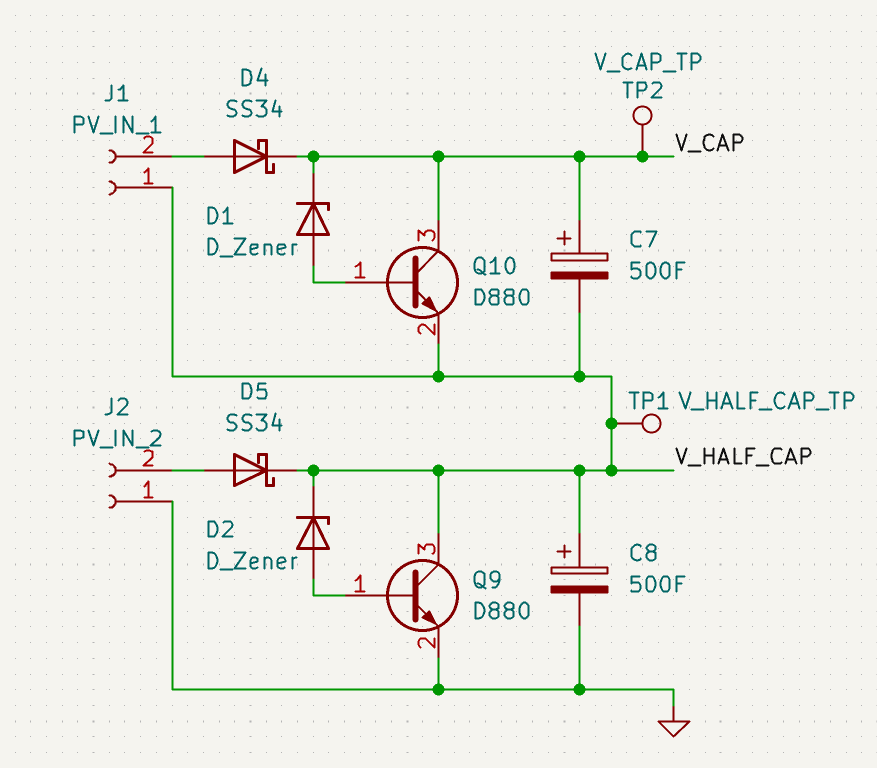
\includegraphics[width=0.9\textwidth]{fig/capacitor_charging_section_zener.png}
        \caption{Sekcja ładowania superkondesatorów z użyciem diod zenera (D1,~D2)}
        \label{rys:cond-charging-zener}
    \end{minipage}\hfill
    \begin{minipage}{0.45\textwidth}
        \centering
        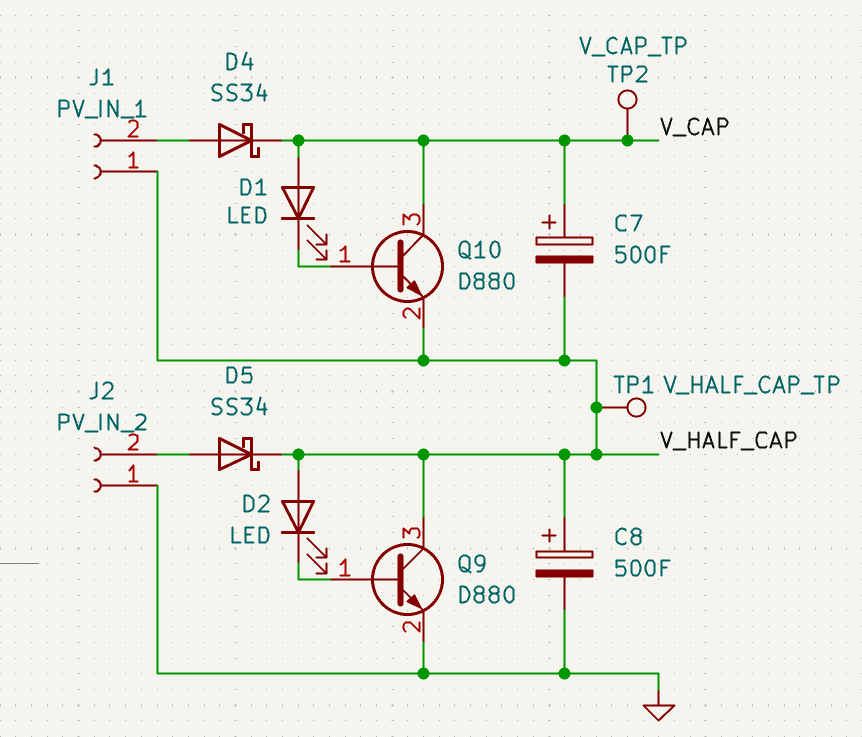
\includegraphics[width=0.9\textwidth]{fig/capacitor_charging_section_led.png}
        \caption{Sekcja ładowania superkondesatorów z użyciem diod LED (D1,~D2)}
        \label{rys:cond-charging-led}
    \end{minipage}
\end{figure}

\begin{table}[h!]
    \centering
    \begin{tabular}{|r|c|c|}
        \hline
        I\textsubscript{E} [mA] & U\textsubscript{Wy} Zener [V]& U\textsubscript{Wy} LED [V] \\
        \hline
        5   & 1,80 & 2,38 \\
        20  & 2,09 & 2,45 \\
        50  & 2,25 & 2,50 \\ 
        100 & 2,40 & 2,53 \\
        200 & 2,65 & 2,57 \\
        500 & 3,00 & 2,68 \\
        \hline
    \end{tabular}
    \caption{Napięcie wyjściowe U\textsubscript{Wy} regulatora bocznikowego przy użyciu diody Zenera i diody LED, dla prądu emitera I\textsubscript{E} tranzystora zwierającego. Do testu użyto zasilacza stałoprądowego.}
    \label{tab:zener-led-voltage-comparison}
\end{table}

\subsection{Układ regulacji napięcia}
Układ regulacji napięcia, przedstawiony na rysunku \ref*{rys:voltage_regulation}, składa się z 2 połączonych ze sobą układów. W celu wykorzystania jak największej ilości energii, zgromadzonej w superkondesatorach, napięcie jest podwyższane poprzez przetwornicę typu step-up --- zbudowaną w oparciu o układ ME210833P --- do wartości 5V. Dzięki temu połączone szeregowo superkondensatory mogą być rozładowane do napięcia mniejszego niż 1V\cite{ME2108A33P}. Podwyższone napięcie jest następnie obniżane do wartości 3.3V z użyciem regulatora liniowego HT7333 o niskim poborze mocy i niskim prądzie spoczynkowym\cite{HT7333}.


\begin{figure}[H]
    \centering
    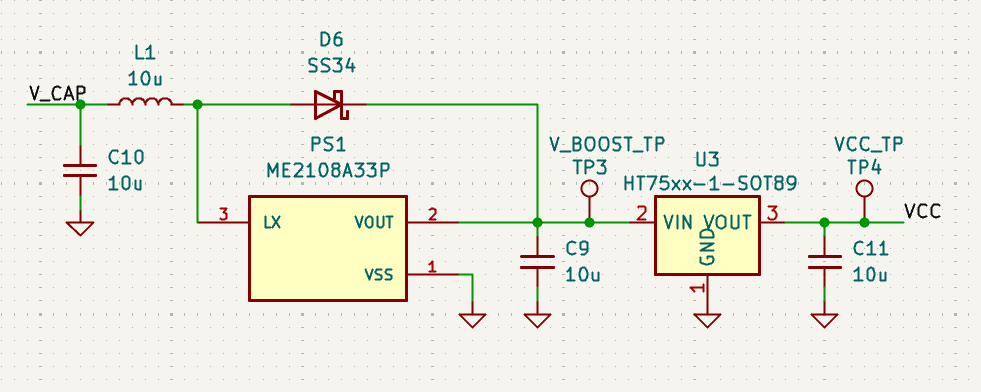
\includegraphics[width=0.9\textwidth]{fig/voltage_regulation_section.png}
    \caption{Układ regulacji napięcia oparty o przetwornicę step-up i regulator liniowy.}
    \label{rys:voltage_regulation}
\end{figure}


\subsection{Magistrala $I^2C$}
\subsection{Mikrokontroler ATmega328p}
\subsection{Układ komunikacji radiowej}

\section{Elementy pomiarowe}
\subsection{Barometr, higrometr i termometr}
\subsection{Moduł z licznikiem Geigera-Müllera}
\subsection{Moduł pomiaru nateżenia światła}

\section{Elementy dodatkowe}
\subsection{Magistrala 1-Wire}
\subsection{Wolne wyprowadzenia GPIO}